\hypertarget{st__resize_8c}{
\section{st\_\-resize.c File Reference}
\label{st__resize_8c}\index{st_resize.c@{st\_\-resize.c}}
}


\subsection{Detailed Description}
\begin{Desc}
\item[For internal use only.]
This file contains the implementation of the \hyperlink{group__dbprim__smat_ga18}{st\_\-resize()} function, used to force a resize of the sparse matrix hash table.\end{Desc}


Definition in file \hyperlink{st__resize_8c-source}{st\_\-resize.c}.

{\tt \#include \char`\"{}dbprim.h\char`\"{}}\par
{\tt \#include \char`\"{}dbprim\_\-int.h\char`\"{}}\par


Include dependency graph for st\_\-resize.c:\begin{figure}[H]
\begin{center}
\leavevmode
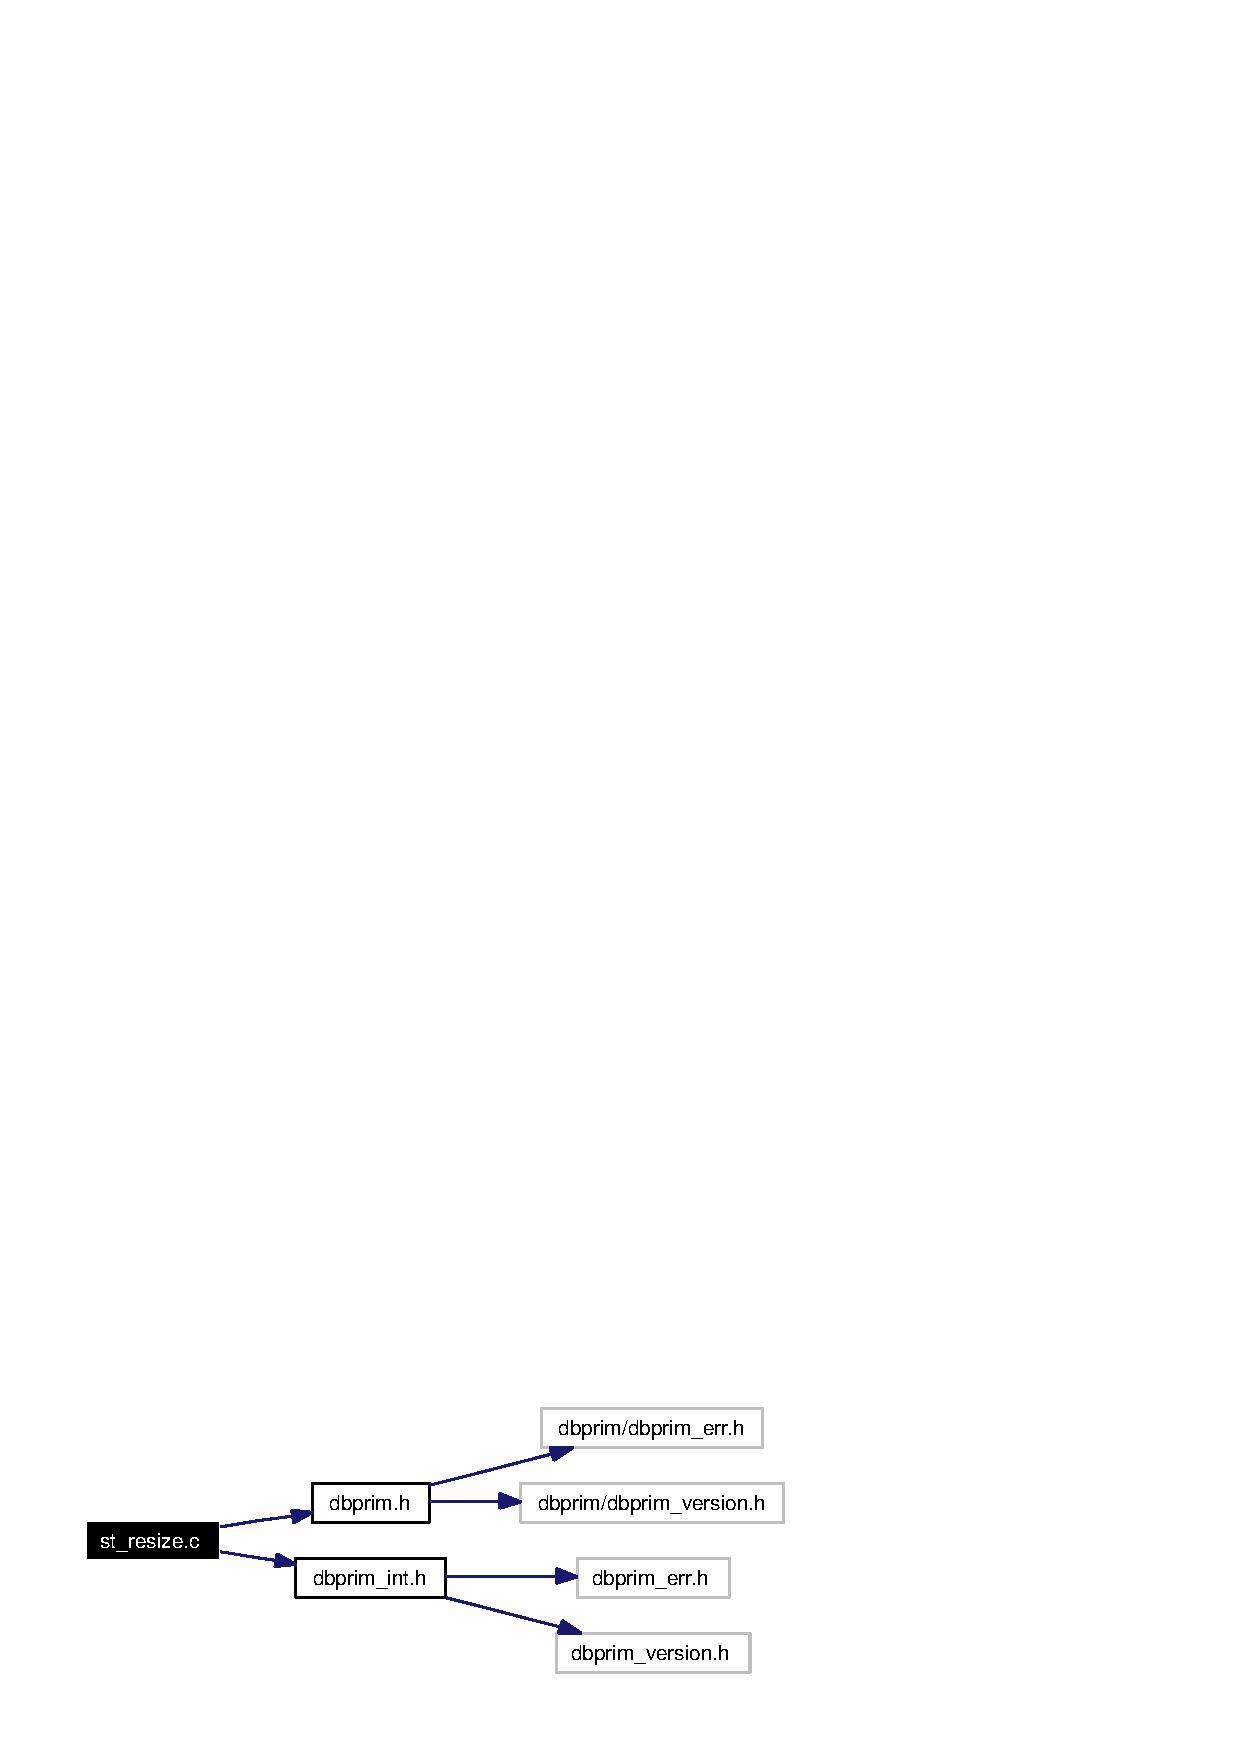
\includegraphics[width=190pt]{st__resize_8c__incl}
\end{center}
\end{figure}
\subsection*{Functions}
\begin{CompactItemize}
\item 
unsigned long \hyperlink{group__dbprim__smat_ga18}{st\_\-resize} (\hyperlink{struct__smat__table__s}{smat\_\-table\_\-t} $\ast$table, unsigned long new\_\-size)
\begin{CompactList}\small\item\em Resize a sparse matrix table. \item\end{CompactList}\end{CompactItemize}
